\documentclass[../structural_economics_book.tex]{subfiles}
\begin{document}
\ifSubfilesClassLoaded{\setcounter{chapter}{16}}{}
\chapter{Domestic Structural Diagnostics}\label{ch:17}
\chaptersubtitle{Reading the National Heatmap}
\begin{quote}
\textit{``La heterogeneidad estructural se manifiesta en la coexistencia de actividades econ\'{o}micas con niveles de productividad correspondientes a distintas \'{e}pocas hist\'{o}ricas.''}\\[0.3em]
\textnormal{[``Structural heterogeneity manifests itself in the coexistence of economic activities with productivity levels corresponding to distinct historical epochs.'']}\\
\hfill --- An\'{i}bal Pinto, ``Naturaleza e implicaciones de la `heterogeneidad estructural' de la Am\'{e}rica Latina'' (1970)
% TODO-VERIFY: wording may be a paraphrase of Pinto's definition; check against El Trimestre Economico 37(145), 1970, and add page.
\end{quote}
\nocite{pinto1970naturaleza}

\vspace{0.3em}

\begin{quote}
\textit{``El casillero vac\'{i}o no es producto del azar ni de la fatalidad: es resultado de la naturaleza del patr\'{o}n de industrializaci\'{o}n vigente.''}\\[0.3em]
\textnormal{[``The empty box is not the product of chance or fate: it is the result of the nature of the prevailing industrialization pattern.'']}\\
\hfill --- Fernando Fajnzylber, ``Industrializaci\'{o}n en Am\'{e}rica Latina'' (1990)
% TODO-VERIFY: not found verbatim; probably not a direct quotation. Check Cuadernos de la CEPAL 60 (1990); if absent, replace with a sourced passage or remove this second epigraph.
\end{quote}
\nocite{fajnzylber1990industrializacion}

\vspace{1em}

Chapter~16 applied the framework at the global scale: the Perron vector of $W^P_{\text{global}}$ measures how concentrated power is among countries, the ECI measures where a country sits in the space of export baskets, and the product space maps the feasible diversification paths. This chapter turns inward: how do you read the structural health of a \textit{national} economy?

The diagnostic toolkit has five instruments, each derived from the weight matrix:
\begin{enumerate}
\item The domestic spectral gap $\Gamma(W^P_{\text{domestic}})$: how integrated are the sectors (how fast do shocks mix)?
\item The between-block variance: how unequal are the blocks?
\item The domestic Perron eigenvector $\boldsymbol{\pi}_{\text{domestic}}$: who has structural power within the country?
\item The domestic $N_{\text{eff}}(W^I)$: how democratic is the information structure?
\item The domestic $\Psi$ ratio: how much does the formation channel matter?
\end{enumerate}

Each instrument is computable from available data: input-output tables, household surveys, media data, and cohort-year panels. Together they provide a structural health check --- a way to diagnose where the economy departs from the benchmark $\Wce = \frac{1}{N}\ones\ones'$ along its two independent coordinates (Chapter~1, Section~\ref{ch01:sec:conventions}): the concentration of power ($G(\boldsymbol{\pi})$, $\Neff$) and the integration deficit ($1 - \Gamma$).

Bolivia is the case study throughout. Two of the five instruments --- $\Gamma$ and the Perron vector of $W^P$ --- are computed here from INE's supply--use tables \citep{ine2026sut}, with comparators from the OECD's Inter-Country Input-Output tables \citep{oecd2023icio,oecd2021icio}; employment comes from ILOSTAT \citep{ilo2026ilostat}, complexity from the Growth Lab \citep{growthlab2026atlas}, and distribution from INE and the World Bank \citep{worldbank2026wdi}. The other three instruments ($\sigma_B$, $\Neff(W^I)$, $\Psi$) need household-survey microdata, audience data and cohort panels that are not used here, and their Bolivian values remain \illustrative. Every number is reproduced by \texttt{code/ch17.py}, which reads the sourced values from \texttt{data/processed}.

The data do not confirm the picture that the structuralist tradition leads one to expect. Bolivia's production network is not unusually fragmented: its $\Gamma$ lies inside the range of Korea, Germany, the United States, Chile, China and Mexico, and its sectoral power is \emph{less} concentrated than theirs. The enclave is real, but it shows up in the Perron weight and the export orientation of hydrocarbons, not in $\Gamma$. Where Bolivia is distinctive is in complexity (a low and falling ECI) and in distribution (a large fall in inequality between 2005 and 2019 while $\Gamma$ stayed roughly flat). The chapter reads the instruments in that light.


%% =====================================================================
\section{Instrument 1: The Domestic Spectral Gap}
\label{ch17:sec:gamma}
%% =====================================================================

\subsection{Estimation from I-O Tables}

\begin{definition}[Domestic Spectral Gap]\label{ch17:def:domestic_gamma}
Let $A$ be the domestic technical-coefficient matrix with the Chapter~1 convention ($a_{ss'}$ = input from sector $s'$ per unit of output of sector $s$; Appendix~\ref{ch17:app:estimation}). The domestic production weight matrix is the matrix of input-cost shares, $W^P = D^{-1}A$ with $D = \operatorname{diag}(A\ones)$:
\begin{equation}\label{ch17:eq:domestic_WP}
W^P_{ss'} = \frac{a_{ss'}}{\sum_{s''} a_{ss''}},
\end{equation}
where $s, s'$ index domestic sectors; every term in row $s$ shares the denominator $X_s$, so the row is sector $s$'s input mix. The \textbf{domestic spectral gap} is $\Gamma(W^P_{\text{domestic}}) = 1 - |\lambda_2(W^P)|$. Report also the normalization used and the level of aggregation: both change $\Gamma$.
\end{definition}

\begin{example}[Bolivia's Domestic $\Gamma$, 2019]\label{ch17:ex:bolivia_gamma}
INE's supply--use tables for 2019 (base 2017), converted to a domestic industry-by-industry table at basic prices and aggregated to the book's 12 sectors. Linkages are column and row sums of $L = (I - A')^{-1}$ computed from the coefficients $A$, so all are at least $1$ and their means coincide. ``Key'' sectors have both normalized linkages ($BL/\overline{BL}$, $FL/\overline{FL}$) at least $1$; ``backward'' or ``forward'' sectors have only one; ``weak'' sectors have neither:

\begin{center}
\begin{tabular}{lcccc}
\toprule
Sector & Output share & $BL$ & $FL$ & Type \\
\midrule
Hydrocarbons & 0.047 & 1.34 & 1.20 & Weak \\
Mining & 0.045 & 1.36 & 1.30 & Weak \\
Public administration & 0.107 & 1.24 & 1.02 & Weak \\
Manufacturing & 0.208 & 1.86 & 2.21 & Key sector \\
Construction & 0.093 & 1.57 & 1.13 & Backward \\
Commerce & 0.078 & 1.42 & 1.58 & Forward \\
Transport & 0.063 & 1.54 & 1.52 & Key sector \\
Financial services & 0.041 & 1.43 & 1.57 & Forward \\
Agriculture & 0.084 & 1.55 & 1.70 & Key sector \\
Other services & 0.144 & 1.36 & 2.02 & Forward \\
Personal services & 0.087 & 1.66 & 1.10 & Backward \\
Domestic services & 0.004 & 1.00 & 1.00 & Weak (no intermediate flows) \\
\midrule
Average & & 1.44 & 1.44 & \\
\bottomrule
\end{tabular}
\par\footnotesize Source: INE, Cuadros de Oferta y Utilizaci\'{o}n 2019, base 2017 \citep{ine2026sut}; domestic flows by import proportionality, basic prices, fixed product-sales structure (Eurostat model D); author's calculations (\texttt{data/compute/compute\_bolivia\_io.py}, \texttt{code/ch17.py}).
\end{center}

Domestic services (households as employers) neither buy nor sell intermediate inputs, so their row of $W^P$ is undefined; $W^P$ is $11 \times 11$. Its spectrum:
\begin{itemize}
\item $\lambda_1 = 1$ (row-stochastic).
\item $\lambda_2 = 0.533$ (real) and $|\lambda_3| = 0.313$: no eigenvalue close to $1$, so there is no sign of weakly coupled blocks at this level of aggregation.
\item $\Gamma = 1 - 0.533 = 0.467$.
\end{itemize}

Bolivia's domestic $\Gamma = 0.467$ is not small. The number depends on the normalization and the aggregation: normalized as sales shares (rows = sellers) the same flows give $\Gamma = 0.694$; at INE's 39-industry detail, input shares give $0.410$. Across the two aggregations, input or sales shares, and with or without the diagonal, Bolivia's 2019 $\Gamma$ ranges over $0.33$--$0.69$. Any single $\Gamma$ used to compare economies should be read against that range.

For comparison on a like-for-like basis (the same 12 groups built from ISIC Rev.~4, domestic flows, input shares, 2019), Bolivia's $\Gamma = 0.475$; South Korea's is $0.511$, Germany's $0.544$, the United States' $0.463$, Chile's $0.557$, China's $0.582$ and Mexico's $0.649$ \citep{oecd2023icio}. Bolivia sits inside the comparator range, above the United States. Aggregate $\Gamma$ does not separate Bolivia from the industrial economies.
\end{example}

\begin{vizpanel}{Domestic $W^P$, 2019: Bolivia and South Korea}
\begin{center}
%% Colour intensity = 100 * W_ij / max(W), rows = buyers, columns = suppliers; from code/ch17.py (HEAT_BOL, HEAT_KOR)
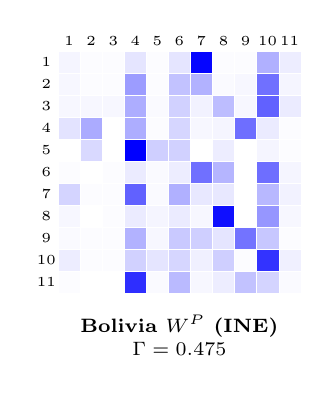
\begin{tikzpicture}[scale=1]
\def\N{11}
\def\s{0.28}
\foreach \i/\j/\bp in {1/1/4,1/2/1,1/3/1,1/4/10,1/5/1,1/6/10,1/7/98,1/8/1,1/9/1,1/10/31,1/11/7,2/1/3,2/2/1,2/3/1,2/4/39,2/5/1,2/6/24,2/7/30,2/8/2,2/9/3,2/10/56,2/11/4,3/1/3,3/2/3,3/3/3,3/4/32,3/5/2,3/6/18,3/7/5,3/8/26,3/9/3,3/10/62,3/11/8,4/1/11,4/2/33,4/3/0,4/4/32,4/5/1,4/6/16,4/7/3,4/8/4,4/9/57,4/10/8,4/11/1,5/1/0,5/2/15,5/3/0,5/4/100,5/5/19,5/6/18,5/7/0,5/8/7,5/9/0,5/10/4,5/11/1,6/1/1,6/2/0,6/3/1,6/4/8,6/5/2,6/6/7,6/7/56,6/8/29,6/9/0,6/10/57,6/11/4,7/1/17,7/2/1,7/3/1,7/4/62,7/5/2,7/6/31,7/7/9,7/8/9,7/9/0,7/10/28,7/11/5,8/1/3,8/2/0,8/3/1,8/4/8,8/5/4,8/6/8,8/7/3,8/8/94,8/9/0,8/10/41,8/11/3,9/1/2,9/2/1,9/3/1,9/4/30,9/5/3,9/6/21,9/7/19,9/8/10,9/9/55,9/10/22,9/11/1,10/1/7,10/2/1,10/3/1,10/4/18,10/5/10,10/6/16,10/7/6,10/8/19,10/9/1,10/10/80,10/11/6,11/1/1,11/2/0,11/3/0,11/4/82,11/5/2,11/6/27,11/7/3,11/8/7,11/9/24,11/10/17,11/11/2} {
    \fill[blue!\bp, draw=white, line width=0.06pt]
      ({(\j-1)*\s}, {(\N-\i)*\s}) rectangle +(\s,\s);
}
\foreach \k in {1,...,11} {
  \node[font=\tiny, black] at ({(\k-0.5)*\s}, {\N*\s+0.12}) {\k};
  \node[font=\tiny, black] at (-0.15, {(\N-\k+0.5)*\s}) {\k};
}
\node[below, font=\scriptsize\bfseries] at ({5.5*\s}, -0.15) {Bolivia $W^P$ (INE)};
\node[below, font=\scriptsize] at ({5.5*\s}, -0.5) {$\Gamma = 0.475$};
\end{tikzpicture}
\qquad
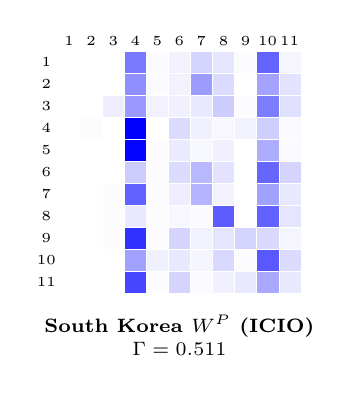
\begin{tikzpicture}[scale=1]
\def\N{11}
\def\s{0.28}
\foreach \i/\j/\bp in {1/1/0,1/2/0,1/3/0,1/4/52,1/5/2,1/6/5,1/7/17,1/8/10,1/9/1,1/10/61,1/11/4,2/1/0,2/2/0,2/3/0,2/4/44,2/5/2,2/6/5,2/7/39,2/8/14,2/9/0,2/10/36,2/11/11,3/1/0,3/2/0,3/3/7,3/4/40,3/5/5,3/6/6,3/7/9,3/8/20,3/9/1,3/10/51,3/11/12,4/1/0,4/2/1,4/3/0,4/4/100,4/5/0,4/6/14,4/7/6,4/8/3,4/9/5,4/10/19,4/11/2,5/1/0,5/2/0,5/3/0,5/4/99,5/5/1,5/6/8,5/7/3,5/8/6,5/9/0,5/10/32,5/11/2,6/1/0,6/2/0,6/3/0,6/4/20,6/5/1,6/6/14,6/7/28,6/8/11,6/9/0,6/10/60,6/11/17,7/1/0,7/2/0,7/3/1,7/4/62,7/5/1,7/6/7,7/7/29,7/8/5,7/9/0,7/10/37,7/11/9,8/1/0,8/2/0,8/3/1,8/4/9,8/5/1,8/6/3,8/7/2,8/8/64,8/9/0,8/10/62,8/11/10,9/1/0,9/2/0,9/3/1,9/4/81,9/5/1,9/6/17,9/7/5,9/8/10,9/9/17,9/10/15,9/11/4,10/1/0,10/2/0,10/3/0,10/4/37,10/5/6,10/6/9,10/7/4,10/8/15,10/9/1,10/10/65,10/11/14,11/1/0,11/2/0,11/3/0,11/4/72,11/5/1,11/6/17,11/7/2,11/8/6,11/9/9,11/10/34,11/11/9} {
    \fill[blue!\bp, draw=white, line width=0.06pt]
      ({(\j-1)*\s}, {(\N-\i)*\s}) rectangle +(\s,\s);
}
\foreach \k in {1,...,11} {
  \node[font=\tiny, black] at ({(\k-0.5)*\s}, {\N*\s+0.12}) {\k};
  \node[font=\tiny, black] at (-0.15, {(\N-\k+0.5)*\s}) {\k};
}
\node[below, font=\scriptsize\bfseries] at ({5.5*\s}, -0.15) {South Korea $W^P$ (ICIO)};
\node[below, font=\scriptsize] at ({5.5*\s}, -0.5) {$\Gamma = 0.511$};
\end{tikzpicture}
\end{center}
\vspace{-0.5em}
\small Row $s$ is sector $s$'s input mix ($W^P = D^{-1}A$, input shares); colour intensity is $W_{ss'}$ relative to each matrix's largest entry (Bolivia $0.60$, construction's purchases from manufacturing; Korea $0.66$, manufacturing's purchases from itself). Sectors: 1~hydrocarbons, 2~mining, 3~public administration, 4~manufacturing, 5~construction, 6~commerce, 7~transport, 8~financial services, 9~agriculture, 10~other services, 11~personal services; domestic services has no intermediate flows and is omitted. Both use the same ISIC-based 12-sector grouping, domestic flows at basic prices. Neither matrix is block-diagonal. In both, the strongest columns are manufacturing (4) and other services (10), the two hubs most sectors buy from; Korea's manufacturing column is stronger still, which is why its Perron vector is more concentrated. Bolivia's hydrocarbons column (1) is nearly white: few domestic sectors buy from it, because 70\% of its output is exported. Its own row is dominated by one supplier, transport. Bolivia's $\Gamma$ is 7\% below Korea's, not 3.5 times below.
\par\footnotesize Sources: INE supply--use tables 2019 \citep{ine2026sut}; OECD ICIO 2023, Korea domestic block \citep{oecd2023icio}; author's calculations (\texttt{code/ch17.py}).
\end{vizpanel}


%% =====================================================================
\section{Instrument 2: Between-Block Variance}
\label{ch17:sec:between}
%% =====================================================================

\begin{definition}[Between-Block Variance]\label{ch17:def:between}
Partition the economy into $k$ blocks (identified from the spectral decomposition of $W^P$ or from sectoral groupings). Let $\bar{y}_b$ be the mean income (or output) per worker in block $b$, $N_b$ the employment in block $b$, and $\bar{y}$ the national average. The \textbf{between-block variance} is:
\begin{equation}\label{ch17:eq:between}
V_B = \sum_{b=1}^k \frac{N_b}{N}(\bar{y}_b - \bar{y})^2.
\end{equation}
The \textbf{between-block share} of total inequality is $\sigma_B = V_B / V_{\text{total}}$. Measured with income it describes income inequality; measured with output per worker it is closer to Pinto's productivity strata. The two need not coincide.
\end{definition}

\begin{proposition}[Between-Block Share as Structural Inequality]\label{ch17:prop:between}
Let $N$ individuals with incomes $y_i$ be partitioned into blocks of sizes $N_b$, with block means $\bar y_b$, overall mean $\bar y = \frac1N\sum_i y_i$, $V_B$ as in~\eqref{ch17:eq:between}, and within-block variance $V_W = \sum_b \frac{N_b}{N}\cdot\frac{1}{N_b}\sum_{i\in b}(y_i - \bar y_b)^2$. With quadratic utility $U(y) = y - \frac{\kappa}{2}y^2$ (and $\kappa y < 1$ for all $y$, so that $U$ is increasing on the relevant range), the utilitarian loss from dispersion decomposes exactly as
\[
\textstyle\sum_i\big[U(\bar y) - U(y_i)\big] = \frac{\kappa}{2}N(V_B + V_W),
\]
so the between-block part is $L_{\text{block}} = \frac{\kappa}{2}NV_B$ (Chapter~2's $L_{\text{block}}$). With $V_{\text{total}} = V_B + V_W$, the between-block share $\sigma_B$ is the fraction of this loss that is \textbf{between blocks} --- associated with the disconnection of the blocks --- as opposed to \textbf{within blocks}.
\end{proposition}

\begin{proof}
For each $i$, $U(\bar y) - U(y_i) = (1 - \kappa\bar y)(\bar y - y_i) + \frac{\kappa}{2}(y_i - \bar y)^2$, which is exact because $U$ is quadratic. Summing over $i$, the linear term vanishes because $\bar y$ is the mean of the $y_i$. For the quadratic term, write $y_i - \bar y = (y_i - \bar y_b) + (\bar y_b - \bar y)$ for $i$ in block $b$; the cross term sums to zero within each block, so $\sum_i (y_i - \bar y)^2 = \sum_b\sum_{i\in b}(y_i - \bar y_b)^2 + \sum_b N_b(\bar y_b - \bar y)^2 = N(V_W + V_B)$ (the law of total variance).
\end{proof}

When $\sigma_B$ is large: most inequality is between blocks. Transfers \emph{across} blocks (pensions, conditional transfers to rural households) reduce $V_B$ directly; transfers within blocks reduce only $V_W$. What transfers do not change is the productivity gap that regenerates $V_B$ each period; cross-block linkages act on that.

When $\sigma_B$ is small: most inequality is within blocks. The economy's problem is not structural heterogeneity but within-sector inequality (which may still have structural causes at a finer scale).

\begin{example}[Bolivia's Between-Block Inequality \illustrative]\label{ch17:ex:bolivia_between}
Illustrative inputs, of the kind one would compute from Bolivia's Encuesta de Hogares (EH) 2019 (Exercise~\ref{ch17:ex:between}). Three blocks: (1) Hydrocarbons/Mining/Government ($N_1 = 0.08N$, $\bar{y}_1 = 18{,}500$ Bs/month), (2) Formal urban ($N_2 = 0.35N$, $\bar{y}_2 = 5{,}200$ Bs/month), (3) Informal/Rural ($N_3 = 0.57N$, $\bar{y}_3 = 1{,}800$ Bs/month).

National mean: $\bar{y} = 0.08 \times 18{,}500 + 0.35 \times 5{,}200 + 0.57 \times 1{,}800 = 4{,}326$ Bs.

Between-block variance:
\begin{align}
V_B &= 0.08(18{,}500 - 4{,}326)^2 + 0.35(5{,}200 - 4{,}326)^2 + 0.57(1{,}800 - 4{,}326)^2 \\
&= 0.08 \times 200.8M + 0.35 \times 0.76M + 0.57 \times 6.38M \\
&= 16.06M + 0.27M + 3.64M = 19.97M.
\end{align}

Assume a total variance $V_{\text{total}} = 32M$. (The three blocks are a substantive partition, by sector and formality, not one read off $W^P$: at the 12-sector level INE's $W^P$ shows no weakly coupled blocks; Example~\ref{ch17:ex:bolivia_gamma}. If Pinto's strata are present, they cut across sectors.)

Between-block share: $\sigma_B = 19.97/32 = 0.62$. Sixty-two percent of income inequality in this illustration is \textit{between blocks}. Transfers within blocks address only the remaining 38\%; transfers across blocks act on the 62\% directly, but only while they last.

For comparison (illustrative): South Korea's $\sigma_B \approx 0.20$ (most inequality is within sectors); Brazil's $\sigma_B \approx 0.45$ (intermediate); the US's $\sigma_B \approx 0.25$. $\sigma_B$ rises mechanically as the partition is refined, so comparisons require the same number and type of blocks.
\end{example}

\begin{prebisch}[Pinto's heterogeneity measured]
\citet{pinto1970naturaleza} described structural heterogeneity qualitatively: the coexistence of a ``modern pole'' with productivity levels comparable to the industrial countries and a ``primitive stratum'' with colonial-era productivity. The between-block variance puts a number on it.

In the illustration, Bolivia's modern pole (gas/mining/government) has average income 10 times the primitive stratum (informal/rural): $\bar{y}_1/\bar{y}_3 = 18{,}500/1{,}800 = 10.3$. Pinto reported much larger \emph{productivity} gaps between the modern and primitive strata for Latin America as a whole. % TODO-VERIFY: the exact ratio and page in Pinto (1970); the earlier text said 20:1.
Income gaps are smaller than productivity gaps because of transfers, remittances and self-employment income. The between-block share $\sigma_B = 0.62$ says that most of this inequality is between strata. Cross-block transfers can reduce it while they last; durable reduction requires structural change: cross-block linkages that equalize productivity across blocks.
\end{prebisch}


%% =====================================================================
\section{Instrument 3: The Domestic Perron Eigenvector}
\label{ch17:sec:perron}
%% =====================================================================

\begin{definition}[Domestic Power Distribution]\label{ch17:def:domestic_pi}
The \textbf{domestic power distribution} is the left Perron eigenvector $\boldsymbol{\pi}$ of the domestic composite weight matrix $W = \alpha_U W^U + \alpha_P W^P + \alpha_I W^I$. The composite exists only if all three layers are row-stochastic on the \emph{same} node set; in practice $W^P$ is measured on sectors, $W^I$ on media outlets or groups, and $W^U$ on households, so each layer's $\boldsymbol{\pi}$ is reported separately. The \textbf{power Gini} is the Gini coefficient of $\pi_1, \ldots, \pi_N$.
\end{definition}

\begin{example}[Bolivia's Domestic $\boldsymbol{\pi}$, 2019]\label{ch17:ex:bolivia_pi}
The Perron vector of the $11 \times 11$ $W^P$ of Example~\ref{ch17:ex:bolivia_gamma}, with employment shares from ILOSTAT's tabulation of the 2019 household survey. ILOSTAT reports ISIC Rev.~4 sections, so the employment rows are mapped to the book's sectors approximately: it does not separate hydrocarbons from other mining, nor public from private education and health (counted here in other services).

\begin{center}
\small
\begin{tabular}{llccc}
\toprule
Sector & ISIC & Emp.\ share & $\pi_s$ (power) & $\pi_s/\text{share}_s$ \\
\midrule
Hydrocarbons & B & (in B) & 0.039 & --- \\
Mining & B & (in B) & 0.037 & --- \\
\quad\textit{Hydrocarbons and mining} & B & 0.013 & 0.077 & 5.7 \\
Public administration & O & 0.026 & 0.005 & 0.19 \\
Manufacturing & C & 0.112 & 0.159 & 1.42 \\
Construction & F & 0.079 & 0.029 & 0.37 \\
Commerce & G & 0.171 & 0.095 & 0.55 \\
Transport & H & 0.071 & 0.092 & 1.30 \\
Financial services & K & 0.007 & 0.162 & 23.4 \\
Agriculture & A & 0.274 & 0.091 & 0.33 \\
Other services & D,E,J,L--N,P,Q & 0.121 & 0.270 & 2.23 \\
Personal services & I, R, S & 0.107 & 0.021 & 0.20 \\
Domestic services & T & 0.019 & --- (no $W^P$ row) & --- \\
\midrule
Total & & 1.000 & 1.000 & \\
\bottomrule
\end{tabular}
\par\footnotesize Sources: $\pi$: INE supply--use tables 2019, base 2017, domestic, input shares \citep{ine2026sut}; employment: ILOSTAT, DF\_EMP\_TEMP\_SEX\_ECO\_NB, 2019 \citep{ilo2026ilostat}; author's calculations (\texttt{data/compute/compute\_bolivia\_io.py}, \texttt{code/ch17.py}).
\end{center}

Power in Bolivia's production network is spread fairly evenly: $G(\boldsymbol{\pi}) = 0.445$ and $\Neff = 6.48$ of a possible 11. On the like-for-like ISIC basis of Example~\ref{ch17:ex:bolivia_gamma} Bolivia's power Gini is $0.435$, \emph{lower} than South Korea's ($0.658$), Germany's ($0.611$), and those of the United States ($0.614$), Chile ($0.568$), China ($0.622$) and Mexico ($0.608$). The largest weights belong to other services ($0.270$: utilities, communications, real estate, business services), financial services ($0.162$) and manufacturing ($0.159$): the hubs from which most sectors buy their inputs. In Korea manufacturing alone holds $\pi = 0.434$; in Germany other services hold $0.440$. In industrial economies $\boldsymbol{\pi}(W^P)$ concentrates on manufacturing and business-service hubs, so a high power Gini in the production network is a mark of industrial depth, not by itself a sign of oppression.

Hydrocarbons holds $\pi = 0.039$, well below the uniform share $1/11 \approx 0.091$: the export sector sits at the periphery of the domestic network. Agriculture, with $\pi = 0.091$, carries more than twice as much. The power-employment ratio is highest in financial services ($23.4$, with 0.7\% of employment) and in hydrocarbons and mining together ($5.7$, with 1.3\%), and lowest in public administration, personal services and agriculture.
\end{example}

\begin{intuition}[What the power-employment ratio means --- and does not]
Because $\boldsymbol{\pi}$ is computed from domestic input-cost shares, a sector's $\pi_s$ reflects how much of the rest of the economy's intermediate purchases come from it, directly and recursively. Exports, taxes and royalties do not enter $W^P$. That is why hydrocarbons, which matter so much for foreign exchange and public revenue, carry little weight here. In 2019, 70\% of the sector's output was exported; it bought only $0.225$ of domestic intermediate inputs per unit of output (manufacturing: $0.558$); and compensation of employees was 6\% of its value added (INE supply--use tables; author's calculations). This is the enclave of \citet{pinto1970naturaleza} and Prebisch, measured correctly: its rents reach the rest of the economy through the fiscal system (the direct hydrocarbons tax, IDH) and the exchange rate, not through production linkages. The enclave is visible in $\boldsymbol{\pi}$ and in export orientation, not in $\Gamma$.

Dividing by the employment share then mostly measures \emph{capital intensity and labor productivity}: finance, and hydrocarbons and mining, employ few workers per unit of value. The ratio is therefore not a measure of the ``structural privilege'' of an individual worker in those sectors.

The farmer in the altiplano is the mirror image. Her sector's weight is not small --- agriculture supplies a third of manufacturing's domestic intermediate inputs (food processing) and a seventh of personal services' (restaurants) --- but it is shared among 27\% of the workforce, so its power-employment ratio is $0.33$.

If sectoral $\boldsymbol{\pi}$ is read as bargaining weight (Assumption~7.A), it enters the allocation rule $x_s^* = \Omega/N + (\pi_s - 1/N)\Phi$ (Proposition~\ref{ch07:prop:allocation-rule}), with $N = 11$ sectors, and the gap $\pi_{\text{gas}} - \pi_{\text{agr}} = -0.052$: agriculture, not gas, would receive more than an equal sector share. Per worker the order reverses, because agriculture divides its share among about 21 times as many workers as hydrocarbons and mining combined. Neither reading is a measure of who captures the gas rents. $\boldsymbol{\pi}(W^P)$ records who supplies whom; the distributional reading of $\boldsymbol{\pi}$ belongs to the bargaining layers ($W^U$, $W^I$) of Chapter~7, where Assumption~7.A is a natural postulate.
\end{intuition}


%% =====================================================================
\section{Instrument 4: The Domestic $\Neff(W^I)$}
\label{ch17:sec:neff}
%% =====================================================================

\begin{definition}[Domestic Information Effective Sample Size]\label{ch17:def:domestic_neff}
Given a proxy for the domestic information network $W^I$ (from media data, social network data, or education enrollment data), the \textbf{domestic $N_{\text{eff}}$} is:
\begin{equation}\label{ch17:eq:domestic_neff}
N_{\text{eff}}(W^I) = \frac{1}{\sum_j (\pi^I_j)^2},
\end{equation}
where $\boldsymbol{\pi}^I$ is the Perron eigenvector of $W^I$ (Definition~\ref{ch06:def:neff}). $\Neff$ lies between $1$ and the number of \emph{nodes} of $W^I$. It is therefore only comparable across countries when $W^I$ is built on the same kind and number of nodes (outlets, outlet groups, or population groups), or after dividing by that number.
\end{definition}

\begin{example}[Bolivia's $\Neff$ \illustrative]\label{ch17:ex:bolivia_neff}
Approximating $W^I$ on four nodes --- Bolivia's main media ecosystems --- with illustrative weights:
\begin{enumerate}
\item State media (Radio Patria Nueva, Bolivia TV, Cambio): dominant in the altiplano and valleys. $\pi^I \approx 0.34$.
\item Private commercial media (Unitel, Red Uno, P\'{a}gina Siete, El Deber): dominant in Santa Cruz and urban centers. $\pi^I \approx 0.37$.
\item Community/indigenous media (community radios, e.g.\ the ERBOL network): rural areas. $\pi^I \approx 0.12$.
\item Social media (Facebook, TikTok, WhatsApp): growing, cross-cutting. $\pi^I \approx 0.17$.
\end{enumerate}

\[
\Neff = \frac{1}{0.34^2 + 0.37^2 + 0.12^2 + 0.17^2} = \frac{1}{0.2958} = 3.38 \approx 3.4.
\]

Bolivia's information environment has approximately 3 independent voices out of a maximum of 4 on this node set. Dividing by the population (11.67 million in 2019; \citealp{worldbank2026wdi}) would mix node sets: the population is not the set of nodes of this $W^I$. What the number says is that, at the level of ecosystems, the consensus is dominated by two sources.

Two caveats. First, using audience shares $\mathbf{s}$ as $\boldsymbol{\pi}^I$ is exact only if every node attends to the same mix, $W^I = \ones\mathbf{s}'$; that matrix has $\Gamma(W^I) = 1$ (\texttt{code/ch17.py}). Concentration and integration are different questions here too. Second, with more nodes (individual outlets, or regions $\times$ outlets) $\Neff$ would be larger. Illustrative comparisons on outlet-level node sets: the US $\Neff \approx 15$--$20$, Scandinavian countries $\Neff \approx 8$--$12$; these are not comparable with Bolivia's $3.4$ on four ecosystems.
\end{example}


%% =====================================================================
\section{Instrument 5: The Domestic $\Psi$ Ratio}
\label{ch17:sec:psi}
%% =====================================================================

\begin{definition}[Domestic $\Psi$]\label{ch17:def:domestic_psi}
The domestic variance ratio for a target behavior (female LFP, savings, education enrollment) is estimated from the cohort-year decomposition of Chapter~11:
\begin{equation}
\hat{\Psi}_{\text{domestic}} = \frac{\Var(\hat{\delta}_c)}{\Var(\hat{\alpha}_t)},
\end{equation}
where $\hat{\delta}_c$ is the cohort effect and $\hat{\alpha}_t$ is the year effect. Two cautions from Chapter~11 apply. (i) With age effects in the model, linear trends in cohort and year effects are not identified (the age--period--cohort problem), so the ratio depends on the identifying restriction, which must be stated and varied. (ii) The variance ratio equals the formation-to-enforcement ratio $\Psi$ only under additional assumptions (all cohort variation is formation, all year variation is enforcement, a common driving index).
\end{definition}

\begin{example}[Bolivia's $\Psi$ for Self-Employment \illustrative]\label{ch17:ex:bolivia_psi}
Following the hypothetical template of Chapter~11: suppose Bolivia's self-employment rate varies across departments --- nationally it was 68.1\% of employment in 2019 (ILO modelled estimate, \citealp{worldbank2026wdi}); departmental rates require EH microdata --- and that a cohort-year decomposition of EH data (2000--2019), under a stated APC restriction, gives:

$\Var(\hat{\delta}_c) = 0.028$ (cohort component: norms about self-employment differ across generations). $\Var(\hat{\alpha}_t) = 0.018$ (year component: labor market conditions change across time).

$\hat{\Psi} = 0.028/0.018 = 1.56$.

Under the mapping assumptions of Chapter~11, the formation channel (norms transmitted through $W^I$) is 56\% larger than the enforcement channel (prices and labor market conditions). Standard labor market policy (wage subsidies, credit access, training) captures at most $1/(1+1.56) = 39\%$ of the total effect. The majority operates through the formation channel.

\begin{center}
\begin{tabular}{lcc}
\toprule
Behavior & $\hat{\Psi}_{\text{Bolivia}}$ & Dominant channel \\
\midrule
Self-employment & 1.56 & Formation \\
Female LFP & $\approx 1.8$ & Formation \\
Savings rate & $\approx 1.1$ & Formation (slight) \\
Education enrollment & $\approx 0.7$ & Enforcement (slight) \\
\bottomrule
\end{tabular}
\end{center}
\end{example}


%% =====================================================================
\section{The Structural Health Dashboard}
\label{ch17:sec:dashboard}
%% =====================================================================

\begin{definition}[Structural Health Dashboard]\label{ch17:def:dashboard}
The \textbf{structural health dashboard} for a national economy reports five numbers:
\begin{center}
\begin{tabular}{llll}
\toprule
\textbf{Instrument} & \textbf{Symbol} & \textbf{Benchmark} & \textbf{Interpretation} \\
\midrule
Spectral gap & $\Gamma$ & $\to 1$ & Sectoral integration \\
Between-block share & $\sigma_B$ & $\to 0$ & Between-block inequality \\
Power Gini & $G(\boldsymbol{\pi})$ & $\to 0$ & Power concentration \\
Information $\Neff$ & $\Neff(W^I)$ & $\to N$ & Information democracy \\
Formation ratio & $\Psi$ & --- & Formation channel strength \\
\bottomrule
\end{tabular}
\end{center}
Here $N$ in the $\Neff$ row is the number of nodes of $W^I$, and $\Gamma$ measures mixing speed. The first four instruments have clear benchmarks ($\Wce$ has $\Gamma = 1$, uniform $\boldsymbol{\pi}$ and $\Neff = N$; $\sigma_B \to 0$ also requires equal endowments). They measure two independent coordinates --- integration ($\Gamma$) and concentration ($G(\boldsymbol{\pi})$, $\Neff$) --- plus between-block inequality, which depends on endowments as well as on $W$. The fifth ($\Psi$) is descriptive: it tells you how much the formation channel matters, not whether it is ``too large'' or ``too small.''
\end{definition}

\begin{example}[Bolivia's Dashboard, 2019 (partly \illustrative)]\label{ch17:ex:dashboard}
\begin{center}
\begin{tabular}{lcccl}
\toprule
\textbf{Instrument} & \textbf{Bolivia} & \textbf{South Korea} & \textbf{Benchmark} & \textbf{Status} \\
\midrule
$\Gamma$ & 0.475 & 0.511 & 1.00 & data \\
$\sigma_B$ & 0.62 & 0.20 & 0.00 & illustrative \\
$G(\boldsymbol{\pi})$ & 0.435 & 0.658 & 0.00 & data \\
$\Neff(W^I)$ & 3.4 & $\approx 12$ & $N$ & illustrative \\
$\Psi$ (self-employment) & 1.56 & $\approx 0.6$ & --- & illustrative \\
\midrule
\textit{Memo:} ECI (Chapter~16) & $-1.30$ & $1.81$ & --- & data \\
\bottomrule
\end{tabular}
\par\footnotesize Sources: $\Gamma$ and $G(\boldsymbol{\pi})$: domestic $W^P$, input shares, ISIC-based 12 sectors, 2019; INE supply--use tables \citep{ine2026sut} and OECD ICIO 2023 \citep{oecd2023icio}; author's calculations (\texttt{data/compute/}, \texttt{code/ch17.py}). Bolivia's $\Gamma$ ranges over $0.33$--$0.69$ across normalizations (Example~\ref{ch17:ex:bolivia_gamma}). ECI: Growth Lab, HS92 \citep{growthlab2026atlas}. The rows marked illustrative need household-survey microdata, audience data and cohort panels.
\end{center}

The two production-network instruments, now measured, do not place Bolivia far from Korea. Its spectral gap is 7\% below Korea's, and its power Gini is \emph{lower} --- Korea's is 1.5 times Bolivia's, because Korea's input purchases concentrate on its manufacturing hub. On these two instruments Bolivia is not an outlier. Where Bolivia does stand apart is in complexity: its ECI of $-1.30$ against Korea's $1.81$ is a gap of more than three standard deviations of the cross-country distribution. The three remaining rows are illustrative: in them Bolivia's between-block share is 3 times Korea's, its information $\Neff$ about 3.5 times smaller (meaningful only on comparable node sets; Section~\ref{ch17:sec:neff}), and its $\Psi$ ratio 2.6 times larger. Whether those gaps are real is an empirical question that the EH microdata and media data would settle.

The dashboard is the structural physician's chart. It tells you what is wrong, how severe, and where to intervene (Chapter~15's operators target integration, power or output separately) --- and, as here, what is \emph{not} wrong.
\end{example}

\begin{keyinsight}
The instruments are not redundant, and no single number summarizes them. $\Gamma$ measures integration: how fast shocks and signals mix across sectors. $G(\boldsymbol{\pi})$ and $\Neff$ measure concentration of power, which is a different coordinate: any power distribution is compatible with any spectral gap (Proposition~\ref{ch06:prop:gap-power-independent}). A doubly stochastic, weakly coupled economy has $G(\boldsymbol{\pi}) = 0$ and $\Gamma \approx 0$; an economy in which every sector buys from one dominant supplier has $\Gamma \approx 1$ and high $G(\boldsymbol{\pi})$. $\sigma_B$ adds endowments and productivity. $\Psi$ measures how much any departure feeds back into preference formation.

Bolivia's measured numbers make the point concrete: an economy with a low and falling ECI and a textbook export enclave has a production-network $\Gamma$ and $G(\boldsymbol{\pi})$ within the range of industrial economies. Aggregate $\Gamma$ does not separate development paths, and a concentrated $\boldsymbol{\pi}(W^P)$ is as much a sign of industrial hubs as of exclusion. The dashboard is useful precisely because the instruments respond to different operators: $\Gamma$ responds most to cross-block $\Delta W^P$ (structural policy); $G(\boldsymbol{\pi})$ to who supplies whom; $\Neff$ to $\Delta W^I$ (information policy); $\Psi$ tells you which lever matters most.
\end{keyinsight}

\begin{vizpanel}{Structural health: Bolivia vs.\ South Korea (bar chart)}
\begin{center}
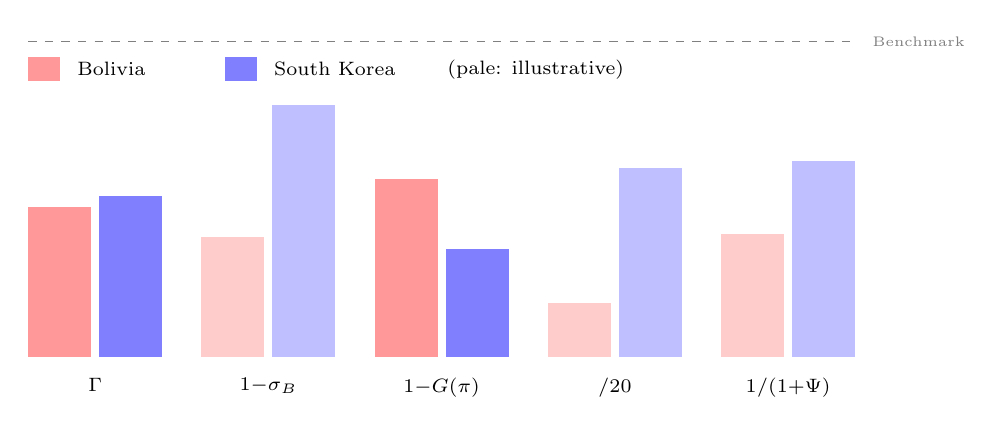
\begin{tikzpicture}[scale=1]
%% Spider/radar chart approximation with bar pairs (values: code/ch17.py, "Dashboard bars")
%% Bolivia bars
\fill[red!40] (0, 0) rectangle (0.8, {0.475*4});
\fill[red!20] (2.2, 0) rectangle (3.0, {0.38*4});
\fill[red!40] (4.4, 0) rectangle (5.2, {0.565*4});
\fill[red!20] (6.6, 0) rectangle (7.4, {0.17*4});
\fill[red!20] (8.8, 0) rectangle (9.6, {0.39*4});
%% Korea bars
\fill[blue!50] (0.9, 0) rectangle (1.7, {0.511*4});
\fill[blue!25] (3.1, 0) rectangle (3.9, {0.80*4});
\fill[blue!50] (5.3, 0) rectangle (6.1, {0.342*4});
\fill[blue!25] (7.5, 0) rectangle (8.3, {0.60*4});
\fill[blue!25] (9.7, 0) rectangle (10.5, {0.62*4});
%% Labels
\node[font=\scriptsize, below] at (0.85, -0.15) {$\Gamma$};
\node[font=\scriptsize, below] at (3.05, -0.15) {$1{-}\sigma_B$};
\node[font=\scriptsize, below] at (5.25, -0.15) {$1{-}G(\pi)$};
\node[font=\scriptsize, below] at (7.45, -0.15) {$\Neff/20$};
\node[font=\scriptsize, below] at (9.65, -0.15) {$1/(1{+}\Psi)$};
%% Legend
\fill[red!40] (0, 3.5) rectangle (0.4, 3.8);
\node[font=\scriptsize, right] at (0.5, 3.65) {Bolivia};
\fill[blue!50] (2.5, 3.5) rectangle (2.9, 3.8);
\node[font=\scriptsize, right] at (3.0, 3.65) {South Korea};
\node[font=\scriptsize, right] at (5.2, 3.65) {(pale: illustrative)};
%% Benchmark line
\draw[dashed, gray] (0, 4) -- (10.5, 4);
\node[font=\tiny, gray, right] at (10.6, 4) {Benchmark};
\end{tikzpicture}
\end{center}
\vspace{-0.5em}
\small Values from Example~\ref{ch17:ex:dashboard} (\texttt{code/ch17.py}); dark bars are data (2019, INE and OECD ICIO, like-for-like), pale bars are illustrative. The first four instruments are rescaled so that the benchmark is 1.0 (top); $\Neff$ is divided by 20 as a common scale, which presumes comparable node sets. The fifth bar, $1/(1+\Psi)$, is the enforcement share and has no benchmark: it is shown for scale only. On the measured instruments Bolivia and Korea are close on integration, and Bolivia is \emph{closer} to the benchmark on power concentration. The gaps measure different things --- integration, between-block inequality, power concentration, information concentration --- and should not be added up.
\end{vizpanel}


%% =====================================================================
\section{Structural Change Over Time}
\label{ch17:sec:time}
%% =====================================================================

\begin{definition}[Tracking Structural Health]\label{ch17:prop:tracking}
The dashboard can be computed for multiple years to track structural change. The trajectory of $(\Gamma_t, \sigma_{B,t}, G(\boldsymbol{\pi}_t), N_{\text{eff},t})$ over time reveals whether the economy is integrating or fragmenting ($\Gamma_t$), and whether power is concentrating or dispersing ($G(\boldsymbol{\pi}_t)$, $N_{\text{eff},t}$).
\end{definition}

\begin{example}[Bolivia 1990--2019: Structural Trajectory]\label{ch17:ex:trajectory}
INE publishes input-output tables for 1988--2009 and 2011--2014 (base 1990) and supply--use tables for 2017--2024 (base 2017). Each year is processed as in Example~\ref{ch17:ex:bolivia_gamma} (book's 12 sectors, domestic flows, input shares):

\begin{center}
\begin{tabular}{llcccc}
\toprule
Year & Base & Sectors in $W^P$ & $\Gamma$ & $G(\boldsymbol{\pi})$ & $\pi_{\text{hydrocarbons}}$ \\
\midrule
1990 & 1990 & 10 & 0.567 & 0.420 & 0.037 \\
2000 & 1990 & 10 & 0.494 & 0.420 & 0.036 \\
2006 (nationalization) & 1990 & 11 & 0.518 & 0.424 & 0.064 \\
2011 & 1990 & 11 & 0.478 & 0.369 & 0.088 \\
2013 & 1990 & 11 & 0.484 & 0.371 & 0.085 \\
\midrule
2017 & 2017 & 11 & 0.506 & 0.446 & 0.045 \\
2019 & 2017 & 11 & 0.467 & 0.445 & 0.039 \\
\bottomrule
\end{tabular}
\par\footnotesize Source: INE, Matrices de Insumo Producto (base 1990) and Cuadros de Oferta y Utilizaci\'{o}n (base 2017) \citep{ine2026sut}; author's calculations (\texttt{data/compute/compute\_bolivia\_io.py}, \texttt{code/ch17.py}). The change of base (rule) brings a new classification and SNA vintage: do not compute changes across it. In 1990 and 2000 the table has no intermediate sales of public administration, so $W^P$ has 10 sectors. There is no table for 2010.
\end{center}

The data tell a story of slow \textit{dis}integration, not of an integrating economy. On base 1990, $\Gamma$ fell from $0.567$ (1990) to $0.484$ (2013), a structural velocity of $-0.036$ per decade. On base 2017 it fell again, from $0.506$ (2017) to $0.467$ (2019). Korea's $\Gamma$ also fell, from $0.626$ (1995, OECD ICIO 2021 edition) to $0.511$ (2019, 2023 edition). Over the period in which one economy became an industrial power and the other remained a commodity exporter, their aggregate $\Gamma$ moved in the same direction. Power in $W^P$ did not concentrate either: $G(\boldsymbol{\pi})$ was $0.42$ in 1990 and $0.37$ in 2013. What moved was the weight of hydrocarbons, which more than doubled with the gas boom, from $0.037$ (1990) to $0.088$ (2011), close to the uniform share $1/11 \approx 0.091$, and stood at $0.039$ in 2019 on the new base, when 70\% of the sector's output was exported.

The other two coordinates cannot be tracked with the data used here: $\sigma_B$ needs EH microdata and $\Neff(W^I)$ audience data. Illustratively, $\sigma_B$ might have fallen from about 0.68 to 0.62 and $\Neff$ risen from about 2.1 to 3.4 (one more independent voice, part of it from social media after 2010) over 1990--2019 \illustrative.

The gas nationalization of 2006 is barely visible in the structural indicators. It changed $\boldsymbol{\omega}$ (revenue distribution) dramatically: the state's take rose sharply --- the hydrocarbons law of 2005 had already raised it to 50\%, and the 2006 decree set 82\% for the largest fields during a transition period. But $\Gamma$ did not jump at 2006: it was $0.502$ in 2005, $0.518$ in 2006 and $0.504$ in 2009. The gas sector remained an enclave in the precise sense of Example~\ref{ch17:ex:bolivia_pi}. The structural diagnosis: Bolivia redistributed within the existing structure without changing the structure.
\end{example}

\begin{prebisch}[The paradox of redistribution without structural change]
Bolivia under Morales (2006--2019) saw one of the largest falls in inequality in the region. Extreme poverty fell from 38.2\% of the population in 2005 to 15.2\% in 2018 (INE's earlier poverty lines; 13.2\% in 2019 on the updated lines). The Gini of per-capita household income fell from $0.600$ (2005) to $0.426$ (2019). GDP growth averaged 4.52\% a year over 2006--2019 (INE, Encuesta de Hogares; \citealp{worldbank2026wdi}). Over the same years $\Gamma$ was roughly flat, drifting down, and the ECI fell from $-1.21$ (2006) to $-1.46$ (2018) and $-1.30$ (2019) \citep{growthlab2026atlas}.

How did inequality fall so much? Decompositions attribute most of the fall to labor income at the bottom of the distribution --- faster earnings growth in low-skill, informal and rural activities during the commodity boom, together with minimum-wage increases --- and a smaller part to public transfers \citep{vargas2015explaining}. Distribution changed a great deal while $W^P$ changed little. This is what the framework predicts once its two coordinates are kept apart: the allocation depends on endowments and on surplus as well as on $\boldsymbol{\pi}$, and $\boldsymbol{\pi}$ is a separate coordinate from $\Gamma$. It is also evidence against any claim that equity gains \emph{require} a high $\Gamma$ or a positive ECI: Bolivia's came with neither rising.

The Fajnzylber diagnosis: by his criterion --- growth \emph{and} equity --- Bolivia came close to the casillero vac\'{i}o during the boom. The structural question is whether it can stay there when commodity prices fall. Fajnzylber's answer, developed in the case study below, is that only a change in the pattern of industrialization (the operators of Chapter~15) makes growth with equity durable; redistribution on an unchanged production structure depends on the price cycle. What the nationalization did not create was not aggregate integration, which Bolivia already had, but linkages from the export enclave into the domestic network and a more complex export basket.
\end{prebisch}


%% =====================================================================
\section{Summary}
\label{ch17:sec:summary}
%% =====================================================================

\begin{enumerate}
\item Five \textbf{diagnostic instruments}: $\Gamma$ (integration), $\sigma_B$ (between-block share), $G(\boldsymbol{\pi})$ (power Gini), $\Neff$ (information concentration), and $\Psi$ (formation ratio). All are computable from available data, once the normalization of $W^P$, the aggregation level, the block partition and the node set of $W^I$ are stated.

\item Bolivia's measured \textbf{production network} is not fragmented: $\Gamma = 0.467$ in 2019 (INE, 12 sectors; $0.33$--$0.69$ across normalizations), inside the range of Korea ($0.511$), Germany ($0.544$) and the United States ($0.463$) on a like-for-like basis, and its power Gini ($0.435$) is lower than theirs. The enclave is measured by $\boldsymbol{\pi}$ and export orientation: hydrocarbons hold $\pi = 0.039$ while exporting 70\% of output. Bolivia is distinctive in complexity (ECI $-1.30$). The other instruments remain illustrative: $\sigma_B = 0.62$, $\Neff = 3.4$ on four ecosystems, $\Psi = 1.56$.

\item \textbf{Structural change is slow, and $\Gamma$ drifted down}: from $0.567$ (1990) to $0.484$ (2013) in Bolivia, as Korea's fell from $0.626$ (1995) to $0.511$ (2019). Aggregate $\Gamma$ does not separate development paths. Meanwhile inequality fell sharply (Gini $0.600 \to 0.426$, 2005--2019), mainly through labor income at the bottom: equity gains did not require a rising $\Gamma$ or ECI. The gas nationalization changed revenues but not structure.

\item The instruments are \textbf{not redundant}: integration ($\Gamma$) and power concentration ($G(\boldsymbol{\pi})$, $\Neff$) are independent coordinates, and $\sigma_B$ also depends on endowments. No single number --- in particular not $\Gamma$ --- summarizes the distance from $\Wce$.

\item \textbf{Policy diagnostic}: compare each instrument to its benchmark, and choose the operator that acts on that instrument (Chapter~15), in the conjectured $\Psi$-ordered sequence.
\end{enumerate}


%% =====================================================================
\section{Exercises}
\label{ch17:sec:exercises}
%% =====================================================================

\begin{enumerate}[label=\textbf{17.\arabic*}, leftmargin=3em]

\item \textbf{Compute Bolivia's $\Gamma$.} Download Bolivia's supply--use or input--output tables from INE (Bolivia is not a separate economy in OECD ICIO). Build $A$ with the Chapter~1 convention (Appendix~\ref{ch17:app:estimation}) and aggregate to 8--12 sectors. Construct $W^P = D^{-1}A$. Compute the eigenvalues, $\Gamma$ and $\boldsymbol{\pi}$. Repeat with the sales-share normalization and with a different aggregation. How much do $\Gamma$ and $G(\boldsymbol{\pi})$ change? Compare with Example~\ref{ch17:ex:bolivia_gamma} and with the range $0.33$--$0.69$.

\item \textbf{Between-block variance.}\label{ch17:ex:between} Using Bolivia's EH 2019:
\begin{enumerate}
\item Define three blocks (gas/mining/government, formal urban, informal/rural).
\item Compute $\bar{y}_b$ for each. Compute $V_B$ and $\sigma_B$.
\item Now try two blocks (formal/informal) and four blocks (gas, formal manufacturing, urban services, rural). How does $\sigma_B$ change with the number of blocks?
\item Which partition gives the highest $\sigma_B$? Show that refining a partition can never lower $\sigma_B$. What does this tell you about comparing $\sigma_B$ across countries, and about the ``natural'' block structure?
\end{enumerate}

\item \textbf{Power-employment ratio.} Reproduce Example~\ref{ch17:ex:bolivia_pi}:
\begin{enumerate}
\item Compute $\boldsymbol{\pi}$ from the domestic $W^P$.
\item Compute the power-employment ratio $\pi_s/\text{share}_s$ for each sector.
\item Which sector has the highest ratio? Least? How much of the ranking is explained by capital intensity (value added per worker)?
\item A worker moves from agriculture ($\pi/\text{share} = 0.33$) to manufacturing ($\pi/\text{share} = 1.42$). If each sector's share $x_s^* = \Omega/N + (\pi_s - 1/N)\Phi$ (Chapter~7) is divided equally among its workers, by how much does her per-worker allocation change? What does the calculation assume?
\end{enumerate}

\item \textbf{Information democracy.} Estimate $\Neff$ for your country:
\begin{enumerate}
\item Identify the major media outlets / information sources and estimate their audience shares.
\item Approximate $\boldsymbol{\pi}^I$ from audience shares (as a proxy).
\item Compute $\Neff$. How many ``independent voices'' does your country have?
\item Compare with Bolivia's $\Neff = 3.4$, first on the same four-ecosystem node set, then on an outlet-level node set. How does the comparison change?
\end{enumerate}

\item \textbf{Bolivia's structural trajectory.} Reproduce Example~\ref{ch17:ex:trajectory} from INE's tables (base 1990: 1988--2009 and 2011--2014; base 2017: 2017--2024), then extend it with EH data:
\begin{enumerate}
\item Compute $\Gamma$, $G(\boldsymbol{\pi})$ and $\pi_{\text{hydrocarbons}}$ for every available year. Which years look like outliers (try 2014), and why must changes not be computed across the change of base?
\item Compute $\sigma_B$ for 2000, 2005, 2010, 2015, 2019. Plot the trajectory.
\item Is there a structural break at 2006 (nationalization)? At 2009 (new constitution)?
\item Project the trend forward: at the current rate, when will $\sigma_B$ fall below 0.40?
\end{enumerate}

\item \textbf{Dashboard comparison.} Choose three Latin American countries (e.g., Bolivia, Chile, Costa Rica). For each:
\begin{enumerate}
\item Estimate $\Gamma$, $\sigma_B$, $G(\boldsymbol{\pi})$ from I-O and household survey data.
\item Estimate $\Neff$ from media data, on a common node set.
\item Plot the three-country dashboard. Which country is structurally healthiest?
\item Using Chapter~15's sequencing framework: what operator would you recommend for the country with the largest structural deficit?
\end{enumerate}

\item \textbf{Bolivia's escape plan.} Synthesize the entire book for Bolivia:
\begin{enumerate}
\item Current position: dashboard from Example~\ref{ch17:ex:dashboard}. ECI $= -1.30$ in 2019, down from $-1.21$ in 2006 (Chapter~16). Product-space position: sparse periphery.
\item Binding constraints: which instrument is furthest from benchmark? Remember that $\Gamma$ (integration) and $G(\boldsymbol{\pi})$ (power) are independent coordinates: an operator that raises $\Gamma$ need not lower $G(\boldsymbol{\pi})$ (Chapter~15).
\item Operator sequence (Chapter~15): information $\to$ institutions $\to$ education $\to$ infrastructure $\to$ ISI-B.
\item Political feasibility (Chapter~14): which coalition would support this sequence? Is the current coalition ($\{M, W\}$ or $\{B, M, W\}$) compatible?
\item Expected trajectory: using the formation model (Chapter~10) with $\rho = 0.85$, $\mu = 0.2$: simulate 30 years. Plot the dashboard trajectory. Bolivia's $\Gamma$ is already in the comparator range (Example~\ref{ch17:ex:bolivia_gamma}): which instrument would you target instead, and how long does it take to move?
\end{enumerate}
\end{enumerate}


%% =====================================================================
\newpage
\section*{Mathematical Appendices}
\addcontentsline{toc}{section}{Mathematical Appendices}
%% =====================================================================


\subsection*{Appendix 17A: Estimating $W^P$ from I-O Tables}
\addcontentsline{toc}{subsection}{Appendix 17A: Estimating $W^P$}
\label{ch17:app:estimation}

\paragraph{The data.} A national I-O table reports $Z_{ss'}$: the intermediate consumption of sector $s$'s output used by sector $s'$ as input (rows are sellers, the usual statistical convention). Total output of sector $s$ is $X_s = \sum_{s'} Z_{ss'} + Y_s$ (intermediate sales + final demand). State whether the table is a supply--use table or a symmetric table, product-by-product or industry-by-industry, domestic or total flows (including imports), and at basic or purchasers' prices: each choice changes $A$.

\paragraph{Technical coefficients.} With the book's Chapter~1 convention (row $s$ is sector $s$'s recipe), the technical coefficient is $a_{ss'} = Z_{s's}/X_s$: the input from $s'$ per unit of output of $s$. The matrix $A = [a_{ss'}]$ is the transpose of the column-normalized table familiar from the statistical convention. Multipliers and linkages are computed from $L = (I - A')^{-1}$.

\paragraph{From $A$ to $W^P$: two normalizations.} (i) \emph{Input shares} (used in this chapter): $W^P_{ss'} = a_{ss'}/\sum_{s''}a_{ss''} = Z_{s's}/\sum_{s''}Z_{s''s}$, the share of sector $s$'s intermediate purchases that comes from $s'$. Every entry of row $s$ shares the denominator, so the row is a probability vector. (ii) \emph{Sales shares}: $B_{ss'} = Z_{ss'}/\sum_{s''}Z_{ss''}$, the share of sector $s$'s intermediate \emph{sales} that go to $s'$. The allocation coefficients $Z_{ss'}/X_s$ themselves are not row-stochastic (rows sum to the intermediate share of output); they must be normalized over intermediate sales. The two normalizations answer different questions --- who depends on whom as a supplier, vs.\ who depends on whom as a customer --- and give different $\Gamma$ and $\boldsymbol{\pi}$: in Example~\ref{ch17:ex:bolivia_gamma}, $\Gamma = 0.467$ vs.\ $0.694$. Report both.

\paragraph{Spectral gap.} Compute the eigenvalues of $W^P$ using standard numerical linear algebra (e.g., \texttt{numpy.linalg.eig} in Python or \texttt{eigen} in R). The spectral gap is $\Gamma = 1 - |\lambda_2|$.

\paragraph{Practical considerations.} (1) I-O tables are typically available at 30--100 sector detail. Aggregating to 8--15 sectors preserves the block structure while reducing noise. (2) The spectral gap is sensitive to small entries: sectors with negligible intermediate flows should be aggregated or excluded, and a sector with none (Bolivia's domestic services) must be dropped, since its row of $W^P$ is undefined. (3) Comparing $\Gamma$ across countries requires comparable sector classifications (ISIC Rev.~4 is standard) and the same level of aggregation, since $\Gamma$ changes with aggregation.


\subsection*{Appendix 17B: Estimating $\sigma_B$ from Household Surveys}
\addcontentsline{toc}{subsection}{Appendix 17B: Estimating $\sigma_B$}
\label{ch17:app:sigma}

\paragraph{The data.} Household surveys (Bolivia's EH, Brazil's PNAD, Mexico's ENIGH) report individual income and sector of employment. Block assignment: classify each individual into a block based on sector, formality status, or geographic location.

\paragraph{Computation.} The between-block variance: $V_B = \sum_b (N_b/N)(\bar{y}_b - \bar{y})^2$. The within-block variance: $V_W = \sum_b (N_b/N)\Var_b(y)$. Total: $V_T = V_B + V_W$. The between-block share: $\sigma_B = V_B/V_T$.

\paragraph{Choice of blocks.} The ``natural'' partition can be identified from the spectral decomposition of $W^P$: when $\lambda_2$ is real, the sign of the second eigenvector $v_2$ partitions sectors into two groups (for non-symmetric $W^P$, use the real part, or the eigenvectors of a symmetrized matrix) (the two sides of the principal axis of differentiation). For $k > 2$ blocks, use $k$-means clustering on the first $k-1$ eigenvectors (spectral clustering). Alternatively, use substantive knowledge (formal/informal, modern/traditional, urban/rural).

\paragraph{Relationship to $\Gamma$.} The between-block share $\sigma_B$ is related to $\Gamma$ through the eigenvalue gap: when $\lambda_2 \approx 1$ (small $\Gamma$, for a reason other than periodicity), the two blocks are nearly independent, and $\sigma_B$ can be large. When $\lambda_2 \ll 1$ (large $\Gamma$), the blocks are integrated, and $\sigma_B$ tends to be small. The relationship is not deterministic: $\sigma_B$ also depends on the endowment distribution, not just the network structure.


%% =====================================================================
\subsection*{Structuralist Case Study: Pinto and Fajnzylber --- Diagnosis and Prognosis}
\addcontentsline{toc}{subsection}{Structuralist Case Study: Pinto (1970) and Fajnzylber (1990)}
%% =====================================================================

This chapter's case study pairs the two structuralist thinkers whose work most directly anticipates the diagnostic toolkit developed here: Pinto's structural heterogeneity (the diagnosis) and Fajnzylber's casillero vac\'{i}o (the prognosis).

\textbf{\citet{pinto1970naturaleza}: The diagnosis.} Pinto's essay ``Naturaleza e implicaciones de la `heterogeneidad estructural' de la Am\'{e}rica Latina'' provided the first systematic description of what this chapter calls the between-block variance. He identified three productivity strata --- primitive, intermediate, and modern --- coexisting within a single economy, with very large productivity gaps between the modern and primitive strata. % TODO-VERIFY: the size of Pinto's reported modern/primitive productivity ratio and its page (earlier drafts said 20:1).
Pinto described the strata, estimated their relative sizes and shares of product, and argued that ISI had failed to integrate them.

In this chapter's notation, Pinto's three strata would correspond to three blocks of $W^P$ with weak cross-block entries ($\Gamma$ small). For Bolivia, INE's tables do not show such blocks at the 12-sector level ($\Gamma = 0.467$, no eigenvalue near $1$; Example~\ref{ch17:ex:bolivia_gamma}). If the strata exist, they lie within sectors --- formal and informal commerce, commercial and peasant agriculture --- and an aggregated $W^P$ cannot see them; $\sigma_B$ from household surveys, or a much finer table, can. His productivity gap corresponds to $\bar{y}_1/\bar{y}_3$ measured with output per worker; measured with income it is smaller. The failure of ISI to integrate the strata corresponds to $\Gamma$ not increasing under ISI (Chapter~15: ISI applied the operator to within-block entries). $\sigma_B$ is an income-based analogue of Pinto's heterogeneity, computable from any household survey; a productivity-based version needs output per worker by stratum.

\textbf{\citet{fajnzylber1990industrializacion}: The prognosis.} Twenty years after Pinto's diagnosis, Fajnzylber asked: what does structural heterogeneity imply for the joint trajectory of growth and inequality? His answer was the casillero vac\'{i}o. In a $2 \times 2$ table of growth (dynamism) against equity, no Latin American country occupied the cell of growth \emph{with} equity: some grew without equity, others had equity without growth. The ``empty box'' was occupied by countries outside the region (South Korea among them) but by no Latin American country.

Fajnzylber's explanation was structural: the prevailing industrialization pattern --- a truncated industrial core without an endogenous capacity for technical progress, led by transnational firms and oriented to imitative consumption --- could not deliver both. His prescription was ``competitividad aut\'{e}ntica'' (genuine competitiveness based on knowledge, technology and institutional quality) as opposed to ``spurious'' competitiveness based on low wages, devaluation or resource extraction --- a distinction he drew in his \citeyear{fajnzylber1988competitividad} article on international competitiveness.

In this chapter's notation, the box requires two things at once, measured by independent instruments: \emph{dynamism}, whose structural basis is an integrated, complex production structure (high $\Gamma$, high ECI, high multipliers), and \emph{equity}, whose structural basis is dispersed power and small between-block gaps (low $G(\boldsymbol{\pi})$, low $\sigma_B$). Because $\Gamma$ and $\boldsymbol{\pi}$ are independent coordinates, neither follows from the other, which is one way to read why the box is hard to enter: a country can move along one coordinate without moving along the other. Bolivia during the gas boom moved toward the box on equity and growth without changing its production structure, and with a falling ECI; Fajnzylber's warning is that such a position is not durable.

The dashboard of this chapter operationalizes Pinto's diagnosis ($\sigma_B$ measures heterogeneity) and gives Fajnzylber's prognosis two measurable coordinates ($\Gamma$ for integration, $G(\boldsymbol{\pi})$ and $\sigma_B$ for equity).

\begin{center}
\begin{tabularx}{\textwidth}{LLL}
\toprule
\textbf{Concept} & \textbf{Pinto (1970)} & \textbf{Fajnzylber (1990)} \\
\midrule
Core claim & Productivity strata coexist & No LA country has growth + equity \\
Formal object & $\sigma_B$ (between-block variance) & Growth $\times$ equity cell \\
Diagnosis & Three strata, $\sigma_B$ large & Casillero vac\'{i}o \\
Mechanism & Weak cross-block linkages in $W^P$ & Truncated industrial core; integration and equity are separate coordinates \\
Dashboard instrument & $\sigma_B$, $G(\boldsymbol{\pi})$ & $\Gamma$, ECI (dynamism); $G(\boldsymbol{\pi})$, $\sigma_B$ (equity) \\
Policy implication & Build cross-block linkages & Raise ECI (``competitividad aut\'{e}ntica'') \\
Bolivia 2019 & $\sigma_B = 0.62$ (illustrative); no blocks visible in $W^P$ & $\Gamma = 0.467$, ECI $= -1.30$ \\
\bottomrule
\end{tabularx}
\end{center}

Pinto diagnosed the disease. Fajnzylber predicted its consequence. This chapter provides the laboratory: five instruments that measure the disease, track its evolution, and identify the structural interventions that could cure it. The instruments are computable from publicly available data (I-O tables, household surveys, trade data, media concentration indices). Any country can run the diagnostic. Run on INE's tables, it does not confirm Pinto's and Fajnzylber's prose in the form one might expect: Bolivia's $\Gamma = 0.467$ and $G(\boldsymbol{\pi}) = 0.445$ are those of an integrated production network with dispersed sectoral power. The heterogeneity they described has to be sought where the data point: in the export enclave (hydrocarbons' $\pi = 0.039$ with 70\% of output exported), in complexity (ECI $-1.30$), and within sectors, which is what $\sigma_B$ from the EH microdata (Exercise~17.2) would measure.


%% =====================================================================
\subsection*{Further Reading}
\addcontentsline{toc}{subsection}{Further Reading}
%% =====================================================================

\textbf{Structural heterogeneity:} \citet{pinto1970naturaleza}, ``Naturaleza e implicaciones de la `heterogeneidad estructural'\,.'' \citet{cepal2010time}, \textit{Time for Equality}, Chapter~2. \citet{infante2009chile}, ``Chile: hacia un desarrollo inclusivo.''

\textbf{The casillero vac\'{i}o:} \citet{fajnzylber1990industrializacion}, ``Industrializaci\'{o}n en Am\'{e}rica Latina: de la `caja negra' al `casillero vac\'{i}o'\,.'' \citet{fajnzylber1983industrializacion}, \textit{La industrializaci\'{o}n trunca de Am\'{e}rica Latina}. \citet{fajnzylber1988competitividad}, ``Competitividad internacional: evoluci\'{o}n y lecciones.'' \citet{cepal2012structural}, \textit{Structural Change for Equality}.

\textbf{Structural diagnostics methods:} CEPAL's Structural Change Index (various publications). UNIDO's Competitive Industrial Performance Index. The Economic Complexity Observatory (\texttt{oec.world}).

\textbf{Bolivia's inequality decline:} \citet{vargas2015explaining}, ``Explaining Inequality and Poverty Reduction in Bolivia.''

\textbf{Bolivia data:} INE (Instituto Nacional de Estad\'{i}stica): I-O and supply--use tables \citep{ine2026sut}, Encuesta de Hogares. ILOSTAT for employment by sector and sex \citep{ilo2026ilostat}; OECD ICIO for comparators \citep{oecd2023icio,oecd2021icio}; the Growth Lab's Atlas data for complexity \citep{growthlab2026atlas}. UDAPE (Unidad de An\'{a}lisis de Pol\'{i}ticas Sociales y Econ\'{o}micas): social indicators. The World Bank's Development Indicators for cross-country comparison.

\end{document}
